\chapter{Configuration and Testing}
\label{configurationandtesting}
This chapter will contain the configuration of all nodes of the concept. In addition the newly developed nodes have to be tested as well as the entire navigation concept.


The structure of this chapter is to address the outer nodes of the navigation concept first and then move to the inner nodes.\\


\section{URDF and Robot State Publisher}

\section{Gazebo}

\subsection{Plugins}

\section{Filter}

\subsection{road\_detection}

\subsection{laser\_filter}

\subsection{robot\_localization}

\subsection{markfreespace}

\section{Cartographer}
The goal of this node is to produce a map that gets more reliable over time.\\

Unfortunately the data available for Cartographer is very self simillar, meaning a straight road will allways look the same and therefore does not have sufficient features for proper loop closure. In contrast to the points from the road detection the lidar can actually supply such features and will therefore be a good improvement for the resulting map.\\

But it is not guaranteed that the lidar will even sees anything the SLAM algorithm has to work with the points of the road detection only aswell.

The basic configuration of cartographer is purely based on the setup of the robot. In this case cartographer is supposed to use lidar and the points of the road detection at the same time. To reduce the amount of times one of the sensor doesn't see anything these will need to be merged in the markfreespace node and cartographer will receive one PointCloud2 only.\\
To improve the map further the odometry supplied by the robot\_localization package is used as an input, aswell as the IMU.

Furthermore cartographer will be set to 2d map building.


\subsection{Tuning}
With the basic configuration cartographer is not able to provide a reliable map and a tuning procedure has to be performed. Here the general recommendation of the tuning guide should be followed, which states to tune local SLAM first and disabling global slam while doing so \cite{cartographertuning}.
To tune the local SLAM the parameter of the tracjectory builder have to be adjusted.\\
The trajectory builder contains a scan-matcher, which will compare incoming sensor data a tries to align it with each other as good as possible. This behavior can be tuned by configuring the size of the linear and angular search windows and the weight for the rotation and translation of the incoming scans.\\
One more important setting is the size of the sub maps. These can be adjusted by the amount of scans they contain. Since the submaps will consist out of the scan matched obstacles it is important to set the size of the submaps not to high, if the incoming data will be very self simillar. Otherwise the scanmatcher will combine too many scans while shifting them over each other since they look so simillar. This results in both rotational and translational error.\\
As soon as the local SLAM produces a reliable result after multiple rounds of the robot the global SLAM can be activated and tuned.\\

The global SLAM has two options of combining the submaps the loop-closure, which will check, if the robot was at this spot already, and a scanmatcher, which will try to match the submaps to the current scan. For both of these the weights can be adjusted individually and like in the local SLAM the size of the window for translation and rotation can be adjusted. Reducing the window size to a minimum is aswell important when dealing with self simillar data, so the submaps will not be shifted on top of each other. The size should be chosen so the global SLAM can still correct errors of the individual submaps 
With these values and the submaps the global planner calculates constraints between the maps which will be valued between 0 and 1. These constraints can be blocked with a threshold value that will block constraints with a smaller value. like this the computation time can be drastically reduced and only the important constraints will be processed. Furthermore the weighting of the Pose of the odometry and the local SLAM can be adjusted, which can be usefull with bad odometry.

\subsection{Testing}
Testing of the SLAM will mostly consist out of a Black-Box Test meaning the only things that will be observed is the output and therefore the map.
The SLAM will be tested in the following cases:
\begin{itemize}
	\item Data purely from the road detection.
	\item Data from road detection and lidar scan with obstacles on the side of the road.
	\item Data from road detection and lidar scan with obstacles on the road.
	\item Long duration test with both road detection and lidar scan with obstacles on the side of the road.
\end{itemize}

During all of these test the navigation will solely work with the predicted goals since it is yet unsure if the SLAM map is even usable. Furthermore the same tuning will be used for all tests.\\

\textbf{Data purely from localization:}\\
The reason for this test is to check if the SLAM algorithm can handle Mapping with as least information as possible. This will make loop-closure difficult and cartographer has to work with the self simillar data only.\\
The aim is, that the robot can drive multiple rounds, on the track and cartographer produces an optimized map with little unmatched submaps and well connected road markings.\\
As long as the localization in the map works nicely the distortion in the map is less important and will not be tested.\\

The following pictures contain the SLAM map after the \nth{1},\nth{3} and \nth{5} round.\\

\todo{include pictures of test}

\textbf{Data purely from localization and lidar scan with obstacles on the side of the road:}\\

\textbf{Data purely from localization and lidar scan with obstacles on the road:}\\
This test is meant to be the worst case for the SLAM algorithm during navigation. The purpose is to check how cartographer handles data loss during obstacle avoidance and lane swapping.
The obstacles will be placed in two corners and therefore in the edge case where the camera has the worst chance of seeing the road because of the steering angle, aswell as on the straight section of the road to cover the case where the camera can not see the road during merging on an other lane. Furthermore the obstacles will be placed far enough apart so the lidar has only vision on one at the same time.\\

\textbf{Long duration test with both road detection and lidar scan with obstacles on the side of the road:}\\
Cartographer seems to not merge old submaps but process all of them allways, which will progressively increase computational load. Since the SLAM is supposed to be used during mapping this can become important with a lot of sensor inputs that offer constraint potential (lidar data) and long runtime.
The same setup as in the \nth{2} test will be used but the focus is on the moment, at which cartographer cannot optimize in real time caused by too many submaps and constraints.\\


\textbf{Discussion of the test results}\\
As proven by the first two tests, cartographer is well tuned and the map would be useable for goal extraction. The submaps are well alligned and the map has no huge translational or rotational offset.\\
The \nth{3} and \nth{4} test on the other hand display the limitations of the slam algorithm.\\
When obstacles are located on the right lane the allignment of the submaps fails and a lot of submaps cant be attached to the rest of the map. After passing the obstacle the map gets better again, which would imply that the map could be good enough for goal extraction, if no obstacle is near the robot.\\
The \nth{4} test proves that cartographer is not usable in SLAM mode during long time navigation an a circuit. This is caused that too many submaps are close to each other that share features for a constraint.

Based on these problems the map will not be used for the navigation for now.
\section{PoseFinder}

\section{Planners}
\section{Costmaps}
Based on the fact that both planners are responsible for different tasks the configuration of the individual costmaps need to fulfill different tasks too. Here we can compare the requirements of the two planners, from which we can determine how the costmaps will be defined.\\

As described in the theoretical knowledge of this thesis the costmap are structured in layers. This means that the data can be evaluated by different plugins before it will be combined into the real costmap.\\

It makes sense to first take a look at the general behaviour, that both planners share. In this case it is obstacle avoidance. This means that the lethal obstacles need to be marked in both costmaps.\\

To realize this the provided plugin obstacle\_layer can be used. It will take incoming sensor data (sensor\_msgs::PointCloud or sensor\_msgs::LaserScan) and mark the points in the costmap.\\

Since the data here comes form the road detection and a lidar and both have a certain resolution it is unsure, if the result of a scanned obstacle in the costmap is actually a closed line or just points, since this highly relies on the resolution of the sensors and the costmap.\\

To fill theses gaps in the costmap the provided plugin inflation\_layer can be used. It will inflate only the lethal obstacles in the costmap with a configurable cost distribution.\\

This setup is already enough for the local costmap, where as the global planner needs to fulfill the quest of changing lanes if necessary but all-ways preferring the right lane. For this a custom plugin will be needed that makes the transition to the left lane more expensive but still possible.

\subsection{dynamic\_cost\_layer}
Enhancing to the plugins provided in the navigation stack this layer handles inflation of cells with a configurable cost decay and radius. While this seems to be similar to the provided inflation layer, this offers way more flexibility since it will inflate specific points by their individual radius and cost distribution and not just every lethal one by one fixed distribution.\\

This behavior can be used to inflate the left road marking in the global costmap to force the global plan on the right side of the road. The plugin can also be used to inflate cells with zero cost, which is useful to guarantee a cost free right lane or to give some free space around obstacles located on the road.\\

The layer receives a message of type sensor\_msgs::PointCloud on a configurable topic. This PointCloud is expected to feature Channel Values for the inflation radius, the maximal and the minimal cost for each individual point.\\

Since we can't assume that the incoming points will be in the frame of the costmap the points in the costmap have to be transformed into the right frame using tf2.\\

To minimize the computation load a bresenham based algorithm for the circle rasterization will be used. Now the point symmetry around the cell can be used to further minimize the computational load and only $\frac{1}{8}$th of the circle has to be computed. The rasterization process can be described by the following image.\\

Adding to the typical behavior of the bresenham rasterization the area of the circle will be filled with the cost specified for the point. For this the following linear decaying \nth{1} degree function will be used which requires the computation of the distance of the rasterized cell to the center of the circle.

\[cost(distance)=maxcost-distance*\frac{maxcost-mincost}{radius}\]\\
with: \[distance=\sqrt{cell.x^2+cell.y^2}\]

 Since this will still require the usage of a square root for each cell in the circle This will be optimized as well.\\

The goal here is to use a function that contains only the squared distance, which still represents a decaying trend. This requirement rules out every function with an odd degree, as well as all functions with an x offset. This leaves all functions with an even degree from which we choose the \nth{2} degree function to reduce square operators. The comparison between the two functions can be seen in the picture below.

\[cost(distance)=maxcost-distance^2*\frac{maxcost-mincost}{radius^2}\]\\
\begin{figure}[h!]
	\begin{center}
	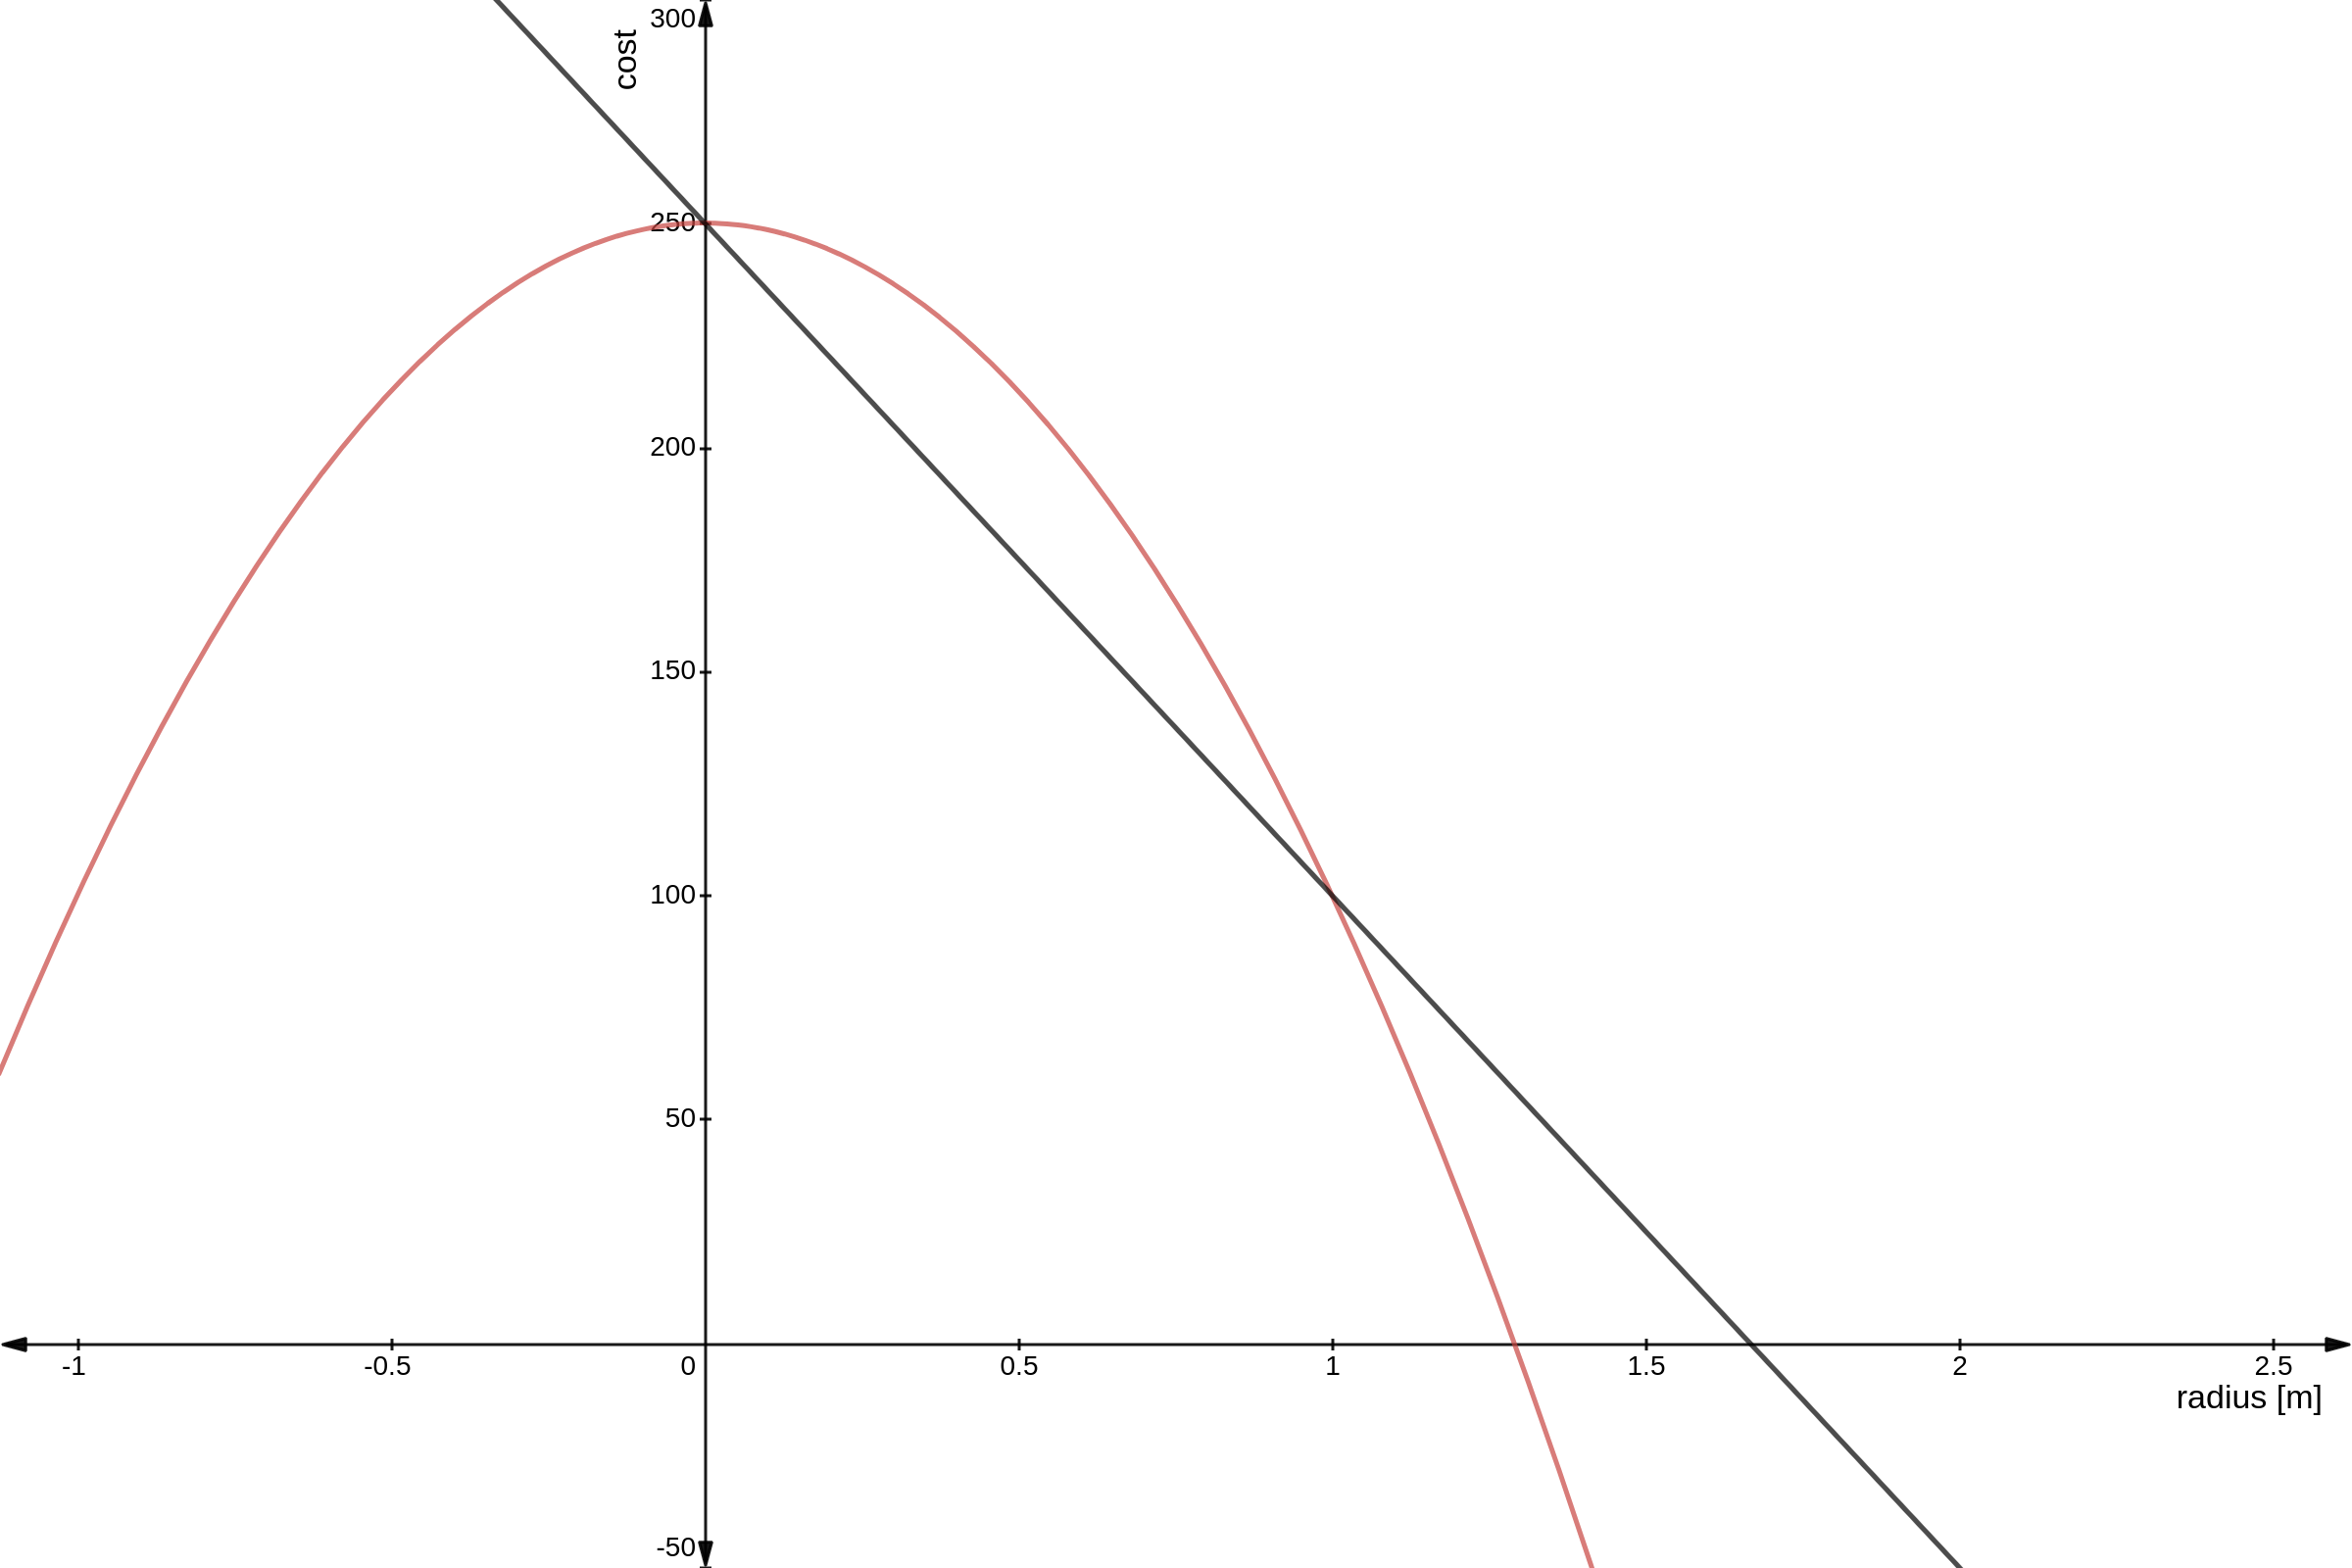
\includegraphics[width=140mm]{Pictures/linear cost comparison}
	\caption{cost distribution comparison with maxcost=250 mincost=100 radius=1}
\end{center}
\end{figure}



\subsection{global\_costmap}

\subsection{local\_costmap}
\subsection{global\_planner}
\subsection{local\_planner}

